\section{Teilversuch 1: Fraunhofer-Beugung am variablen Einfachspalt}
	Als wir die Spaltbreite schrittweise reduzieren, sehen wir erst den Übergang zwischen Fresnel- und Fraunhofer-Beugung und dann die Fraunhofer-Beugung, was wir im Versuch beobachten und erklären sollen.
	\begin{figure}[H]
		\centering
		% https://tex.stackexchange.com/a/473626
		\begin{tabular}{ccc}
			\begin{tabular}{l}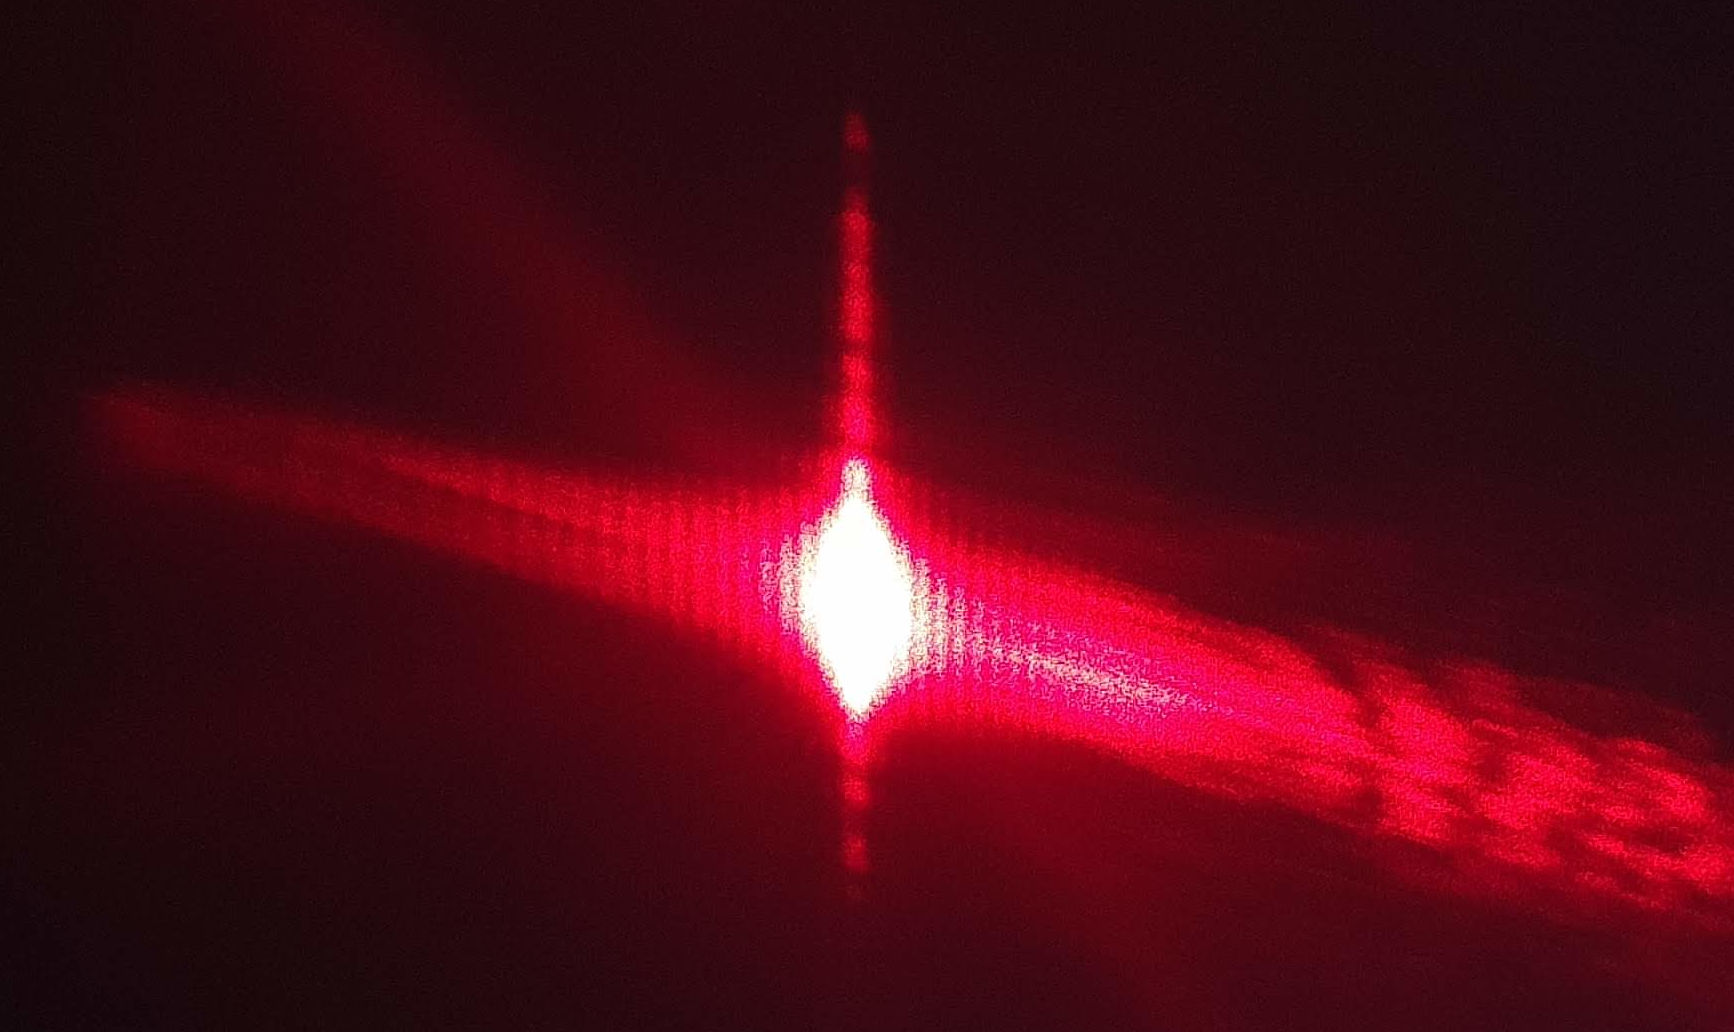
\includegraphics[width=0.4\textwidth]{tv1-fresnel.jpg}\end{tabular} & 
			\begin{tabular}{c}schmaler\\[1em] {\Huge$\rightarrow$}\end{tabular} & 
			\begin{tabular}{l}\includegraphics[width=0.4\textwidth]{tv1-übergang.jpg}\end{tabular}
		\end{tabular}
		\caption{\centering Fresnel-Fraunhofer Übergang}
		\vspace{-1em}
	\end{figure}
	Das Laserlicht war im Versuch zu hell, um das Fresnelsche Beugungsmuster sehen zu können. 

	Im Fall der Fraunhoferschen Beugung erfüllt der Abstand zwischen Quelle und Blende\footnote{in diesem Fall kleiner als der Abstand zwischen Blend und Beobachtungsort} $R$ die Relation:
	\begin{wrapfigure}{r}{0.45\textwidth} 
		\vspace{-10pt}
		\begin{center}
			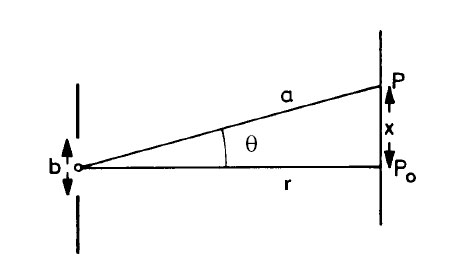
\includegraphics[width=0.4\textwidth]{singleslit.jpg}
			\caption{\textcolor{gray}{Abbildung aus Anleitung BEU Seite 10 §1.6 Abbildung 7 links}}
			\label{fig:singleslit-geo}
		\end{center}
		\vspace{-10pt}
	\end{wrapfigure} 
	\begin{equation}
		R \gg \frac{b^2}{\lambda}
	\end{equation}
	wobei $b$ die Spaltbreite und $\lambda$ die Wellenlänge unseres Lasers ist. Man kann unter dieser Bedingung die Kugelwellen als ebene Wellen annähern und die Lage der Intensitätminima im Beugungsbild durch einfache geometrische Betrachtung bestimmen\footnote{Anleitung BEU Seite 9 §1.6}. Es treten somit Minima auf, wenn es gilt:
	\begin{align}
		b \sin \theta = m \lambda \implies \frac{b}{\lambda}\sin\theta = m && m \in \intzahl
	\end{align}
	Ist nun der Abstand vom Spalt zum Beobachtungspunkt auf dem Schirm $a$ viel größer als der Abstand vom Zentrum der Beugungsmuster zur Beobachtungspunkt $x$, dann ist der Winkel $\theta$ klein und es gilt die Kleinwinkelnäherung mit $\sin\theta \approx \theta$ und wir erhalten:
	\begin{align}
		\frac{b}{\lambda}\theta = m
	\end{align}
	In diesem Fall ist $a$ dann näherungsweise $\approx r$, der Abstand vom Spalt zum Schirm. Im Bogenmaß gilt somit, dass $x = r\theta$ bzw. $\theta = \nicefrac{x}{r}$. Eingesetzt erhalten wir:
	\begin{align}
		\frac{b}{\lambda}\cdot\frac{x}{r} = m \implies x_m = m \cdot \frac{r\lambda}{b}
	\end{align}
	Der Abstand zwischen 2 Minima ist dann gegeben durch:
	\begin{align}
		\Delta x = \frac{r\lambda}{b}
	\end{align}
	die Minima sind also äquidistant, was wir im Versuch auch beobachtet haben.

	Wenn man Spaltbreite verkleinert, war der Beugungsmuster mehr ausgedehnt und der Abstand zwischen die Minima nimmt zu. Das entspricht auch unsere Erwartungen, da $\Delta x$ proportional zu $\frac{1}{b}$ ist. 